\chapter{Fluids Background}
\section{Boussinesq approximation}

The Navier-Stokes equations are the mathematical equations that govern the evolution of fluid flow. In the context of the ocean and atmosphere, the Navier-Stokes equations, along with equations for conservation of mass and energy and an equation of state, provide a good model of the evolution of fluid flow (e.g. Batchelor\cite{batchelor}). For our purposes, however, these equations are too general and an approximation, called the Boussinesq approximation, can be made which results in a simplified version of the Navier-Stokes equations:  
\begin{align} 
\frac{\partial \bm{u}}{\partial t} + \bm{u}\cdot \nabla \bm{u} = -\frac{1}{\rho_{0}}\nabla p - \frac{\rho' g}{\rho_{0}}\hat{\bm{e}}_{z} + \nu \nabla^{2}\bm{u} \label{boussinesq1},\\
\nabla \cdot \bm{u} =0 \label{boussinesq2},\\
\frac{\partial \rho'}{\partial t} + \bm{u}\cdot \nabla \rho' = \kappa \nabla^{2}\rho' - \frac{\partial \bar{\rho}}{\partial z} w,\label{boussinesq3}
\end{align}
where we have the following dimensional variables:
\begin{itemize}
\item $\textbf{u}(x,y,z,t)=(u(x,y,z,t),v(x,y,z,t),w(x,y,z,t))$ is the velocity field in the $x,y,z$-directions respectively,
\item $p(x,y,z,t)$ is the pressure field,
\item $\rho(x,y,z,t)$ is the density,
\item $\rho_{0}$ is a constant reference density,
\item $\bar{\rho}(z)$ is a background density profile,
\item $\rho'(x,y,z,t)=\rho(x,y,z,t)-\bar{\rho}(z)$ is a perturbation density,
\item $g$ is the gravitational constant,
\item $\nu=\mu/\rho_{0}$ is the constant kinematic viscosity,
\item $\mu$ is the constant dynamic viscosity,
\item $\kappa$ is the constant molecular diffusivity.
\end{itemize}
Equations (\ref{boussinesq1})-(\ref{boussinesq3}) are a set of five coupled partial differential equations for the unknowns $\textbf{u},p,\rho$. Herein, we will refer to equation (\ref{boussinesq1}) as the velocity or momentum equations, equation (\ref{boussinesq2}) as the continuity equation, and equation (\ref{boussinesq3}) as the density equation. An additional useful quantity is the buoyancy frequency or the Brunt-V\"ais\"al\"a frequency which is defined as
\begin{align}
N^{2} = -\frac{g}{\rho_{0}}\frac{d\bar{\rho}}{dz}.
\end{align}
Note that we have included a negative sign because we assume that the density profile is decreasing. We now assume that $N$ is constant, which implies a linear background density profile.

A rigorous derivation of the Boussinesq equation is quite delicate and we provide a brief overview of the derivation. A complete derivation, along with many of the subtleties can be found in numerous books such as \cite{batchelor,kundu,tritton,vallis}. The Navier-Stokes equations for a compressible Newtonian fluid can be written as
\begin{align}
\rho \frac{D\bm{u}}{Dt} = -\nabla p - \rho \textbf{g} + \mu \nabla^{2}\bm{u},\\
\frac{1}{\rho}\frac{D\rho}{Dt} + \nabla \cdot \bm{u}=0.\\
\rho c_{p} \frac{DT}{Dt} -\alpha T \frac{D\rho}{Dt}=k\nabla^{2}T+\phi,\label{energy_equation}
\end{align}
where $\alpha=-\rho^{-1}(\partial \rho/\partial T)_{p}$ is the coefficient of thermal expansion, $c_{p}$ is the specific heat, and $\phi$ represent conversion of kinetic energy to internal energy by viscous dissipation\cite{waitecnotes}. To close the system, we need an equation of state, which we take to be \cite{kundu}
\begin{align}
\rho = \rho_{0}(1-\alpha(T-T_{0})).\label{equation_of_state}
\end{align}

The first approximation we make is that of incompressibility. The conditions for incompressibility are \cite{batchelor,kundu,waitecnotes}
\begin{enumerate}
\item Unsteadiness: the time scale of the flow is longer than that of the sound waves.
\item Speed: the characteristic velocity of the flow is much smaller than the speed of sound.
\item Gravity: the vertical scale of the flow is not too large.
\end{enumerate}
Mathematically, letting $v$ denote the speed of sound in the medium, $T$ the characteristic time, $u$ the characteristic velocity, and $L_{v}$ the characteristic vertical length, these three conditions become \cite{waitecnotes}
\begin{align}
\text{unsteadiness: } T^{2} &\gg L^{2}/v^{2},\\
\text{speed: } (u/v)^{2} &\ll 1,\\
\text{gravity: } L_{v}&\ll v^{2}/g.
\end{align} 
For the atmosphere, $v\approx 330$ m/s, $g=9.8 \text{ m/s}^{2}$. The speed condition is easily satisfied if $u< 100$ m/s. The gravity condition holds as long as $L\ll 11 \text{ km}$ which implies that the unsteadiness condition holds as long as $T\gg 30$ s. Such conditions are reasonable for shallow motions in the atmosphere. For the ocean $v\approx 1500$ m/s thus speed is satisfied if $u<475$ m/s, $L<230$ km, and $T>300$ s. Again, such conditions are satisfied in the ocean. Assuming incompressibility, the conservation of mass equation can be approximated as \cite{kundu,waitecnotes}
\begin{align}
\frac{1}{\rho}\frac{D\rho}{Dt} + \nabla \cdot \bm{u}=0 \Rightarrow \nabla \cdot\bm{u}=0.
\end{align}

The Boussinesq equations approximation is made by making the following decomposition of the density \cite{kundu,vallis}
\begin{align}
\rho(\bm{x},t) = \rho_{0} + \bar{\rho}(z) + \rho'(\bm{x},t)\label{bouss_approx}
\end{align}
where we assume that $|\rho'| \ll |\bar{\rho}(z)| \ll |\rho_{0}|$. In other words, variations to the density are small compared to a reference density. Using this approximation and some thermodynamics, Eq (\ref{energy_equation}) simplifies \cite{kundu,vallis} to
\begin{align}
\frac{DT}{Dt} = \kappa\nabla^{2}T.
\end{align}
Plugging in the equation of state (\ref{equation_of_state}) and using (\ref{bouss_approx}) we obtain (\ref{boussinesq3}).

Consider the first two terms in (\ref{bouss_approx}). To these background densities, we associate \cite{kundu,vallis} a corresponding background pressure term in hydrostatic balance so that
\begin{align}
\nabla \bar{p}(z) = -(\rho_{0}\textbf{g} + \bar{\rho}(z)\textbf{g}).\label{bgpressure}
\end{align}

Plugging in (\ref{bouss_approx}) into the momentum equation (\ref{boussinesq1}) and dividing through by $\rho_{0}$ we obtain
\begin{align} 
\left(1 + \frac{\bar{\rho}}{\rho_{0}} + \frac{\rho'}{\rho_{0}}\right)\frac{D\bm{u}}{Dt} = -\frac{1}{\rho_{0}}\nabla p - \left(1 + \frac{\bar{\rho}}{\rho_{0}} + \frac{\rho'}{\rho_{0}}\right)\textbf{g} + \nu \nabla^{2}\bm{u},
\end{align}
and subtracting (\ref{bgpressure}) yields
\begin{align} 
\left(1 + \frac{\bar{\rho}}{\rho_{0}} + \frac{\rho'}{\rho_{0}}\right)\frac{D\bm{u}}{Dt} = -\frac{1}{\rho_{0}}\nabla p' - \frac{\rho'}{\rho_{0}}\textbf{g} + \nu \nabla^{2}\bm{u},
\end{align}
where $p' = p - \bar{p}$. Using $|\rho'|\ll |\bar{\rho}|\ll|\rho_{0}|$, we can neglect the ratios in front of the material derivative to obtain \cite{kundu} (\ref{boussinesq1}). Thus we have derived the Boussinesq equations.

\section{Linear stability analysis}
The study of flow stability has a long and rich history within fluid dynamics. The classic experiment into the stability of fluid flow is that of  Reynolds \cite{reynolds1883}. In this experiment, Reynolds injected dye into the laminar flow through a pipe. By varying the velocity of the flow through the pipe Reynolds observed various effects. If the velocity was sufficiently low, Reynolds was able to observe ``a beautiful straight line through the tube" \cite{reynolds1883}. At slightly higher velocities, the straight line behaviour remained near the initial part of the pipe but further down ``the streak would shift about the tube, but there was no appearance of sinuosity" \cite{reynolds1883}. By increasing the velocity significantly, the dye would again initially remain straight near the initial part of the tube, but instead of shifting about the tube ``the colour band would all at once mix up with the surrounding water, and fill the rest of the tube with a mass of coloured water" \cite{reynolds1883}.

What Reynolds observed was the transition and breakdown of a flow into turbulence. Through careful observation, he determined that the dimensionless quantity that governed the behaviour of the flow was the Reynolds number 
\begin{align}
Re =\frac{UL}{\nu},
\end{align}
a dimensionless number which represents the ratio between the inertial and viscous terms in the Navier-Stokes equations. Reynolds found that if $Re<13000$ then the flow would remain stable \cite{reynolds1883}.

A natural question to ask is whether we can predict such criteria for any given flow. Ideally, given information about a certain flow, one would be like to be able to determine how the fluid will evolve based on various parameters of the flow, such as viscosity, temperature, or velocity. Unfortunately this task has not been achieved in general and there is no known way to determine such criteria for any arbitrary flow.  This is due to the complicated nonlinear behaviour of the Navier-Stokes equations which makes devising a general algorithm for this task incredibly difficult. Tackling this goal in general is immensely difficult and beyond current mathematics, indeed it is not even known whether or not in three dimensions given an initial condition a solution even exists for all times \cite{mill}.

Thus, to proceed, a simplifying approach must be derived. In order to do this, consider the following idea. Let $(\bm{u}_{0},p)$ denote a basic steady state that solves the Navier-Stokes equations and let $(\bm{u}',p')$ denote a small unknown perturbation such that $|\bm{u}',p'|\ll |\bm{u}_{0},p|$. Mathematically this means
\begin{align}
\bm{u}(\bm{x},t) = \bm{u}_{0}(\bm{x}) + \bm{u}'(\bm{x},t),\qquad\label{linear_def} p(\bm{x},t) = p_{0}(\bm{x},t) + p'(\bm{x},t).
\end{align}
Now let us plug (\ref{linear_def}) into the Navier-Stokes equations and expand, dropping the $(\bm{x},t)$ notation,
\begin{align}
\frac{\partial \bm{u}_{0}}{\partial t} + \frac{\partial \bm{u}'}{\partial t} + (\bm{u}_{0}+\bm{u}')\cdot\nabla(\bm{u}_{0}+\bm{u}') = -\frac{1}{\rho_{0}}\nabla(p_{0} + p') + \nu\nabla^{2}(\bm{u}_{0} + \bm{u}'),\label{expanded_lin_NS}\\
\nabla \cdot \bm{u}_{0} + \nabla \cdot \bm{u}'=0.
\end{align} Expanding out the advection term yields
\begin{align}
 (\bm{u}_{0}+\bm{u}')\cdot\nabla(\bm{u}_{0}+\bm{u}') &= \bm{u}_{0}\cdot\nabla\bm{u}_{0} + \bm{u}_{0}\cdot\nabla \bm{u}' + \bm{u}'\cdot\nabla\bm{u}_{0} + \bm{u}'\cdot\nabla\bm{u}'\\
&= \bm{u}_{0}\cdot\nabla\bm{u}_{0} + \bm{u}_{0}\cdot\nabla \bm{u}' + \bm{u}'\cdot\nabla\bm{u}_{0} + \mathcal{O}(\bm{u}'^{2}),
\end{align}
where we have written the $\bm{u}'\cdot\nabla\bm{u}'$ term has $\mathcal{O}(\bm{u}'^{2})$ because this term is of order $\bm{u}'$ squared, which we assume to be small. Now recall that the basic state $\bm{u}_{0}$ solves the Navier-Stokes equations. Thus in (\ref{expanded_lin_NS}) there are terms that depend just on $\bm{u}_{0}$ and they will vanish by definition of it being a solution to the Navier-Stokes equations. Thus we now have that
\begin{align}
\frac{\partial \bm{u}'}{\partial t} + \bm{u}_{0}\cdot\nabla \bm{u}' + \bm{u}'\cdot\nabla\bm{u}_{0} + \mathcal{O}(\bm{u}'^{2})  = -\frac{1}{\rho_{0}}\nabla p' + \nu\nabla^{2}\bm{u}',\\
 \nabla \cdot \bm{u}'=0.
\end{align}
So far, the equation above is exact and we have just written the quadratic nonlinear term in the Big-O notation. Now the critical assumption we make is that because $\bm{u}'$ is small relative to the basic state $\bm{u}_{0}$, $\bm{u}'^{2}$ is even smaller and thus is negligible. In other words, we are throwing away the quadratic nonlinearity of the perturbation term because it assumed to be small. 

Now making the approximation that $\mathcal{O}(\bm{u}'^{2})$ is small we obtain
\begin{align}
\frac{\partial \bm{u}'}{\partial t} + \bm{u}_{0}\cdot\nabla \bm{u}' + \bm{u}'\cdot\nabla\bm{u}_{0} =  -\frac{1}{\rho_{0}}\nabla p' + \nu\nabla^{2}\bm{u}',\\
 \nabla \cdot \bm{u}'=0.
\end{align}
The above set of equations is linear which means they are more amenable to analytical and numerical techniques. 

To illustrate the usefulness in this approach, we demonstrate an example of the general idea of linear stability and apply it to the formulation of the plane parallel shear flow. This is a standard example and we follow the derivation of \cite{drazinreid}. It will also elucidate the key features of linear stability analysis that we will use throughout this thesis.

The first simplifying assumption we make is that the basic state $\bm{u}_{0}=U(z)\hat{\bm{e}}_{x}$, a parallel shear flow, which simplifies the above equations to
\begin{align}
\frac{\partial \bm{u}'}{\partial t} + U\frac{\partial \bm{u}}{\partial x} + w'\frac{dU}{dz}\hat{\bm{e}}_{x}= -\frac{1}{\rho_{0}}\nabla p' + \nu\nabla^{2} \bm{u}',\\
\nabla \cdot\bm{u}'=0.
\end{align}
If we had considered the Euler equations instead of the Navier-Stokes equations, we would have the same equations as above except with $\nu=0$. Despite this seemingly simple modification, the resulting equation is very different. When the inviscid equations are considered, there are many elegant results about the stability of the flow that can be derived for the special case of parallel shear flow. For example, the Rayleigh's inflection point theorem states that a necessary condition for instability is that the basic velocity profile should have an inflection point\cite{drazinreid}. Unfortunately, many of the results for inviscid flow theory do not hold for viscous flow theory. A complete discussion of this result and its generalisation, among other theorems, can be found in \cite{drazinreid,kundu}.

Since the resulting set of equations is a set of coupled linear equations, the solution set involves complex exponentials. Thus, the next natural step is to expand the solution as Fourier modes  
\begin{align}
\bm{u}'(\bm{x},t) = \hat{\bm{u}}(z)e^{i(\alpha x +\beta y -\alpha ct)},\\
p'(\bm{x},t) = \hat{p}(z)e^{i(\alpha x +\beta y -\alpha ct)},
\end{align}
where we take the real part of the above solutions. We require that the solution remains bounded as $x,y\Rightarrow\pm\infty$ which means that $\alpha,\beta$ must remain real. For $c$, however, we let it remain an arbitrary complex number $c=c_{r} + ic_{i}$. Depending on the sign of $c_{i}$ the result will either decay or grown exponentially as time goes to infinity. We thus associate stability with $c_{i}\le 0$ and instability with $c_{i}>0$. Hence, if we are able to solve the above system and derive a criteria for the value of $c_{i}$ we will be able to derive some criteria for the stability of the flow.

Plugging in the above Fourier expansions into the linear equations would yield an eigenvalue-eigenvector problem with $c$ being the undetermined eigenvalue as a function of $\alpha,\beta,Re$. From there we could apply numerical linear algebra routines to solve numerically for various $Re,\alpha,\beta$ and obtain a stability curve for $c$. However, a result due to Squire allows us to simplify the problem significantly. Squire's theorem states that to obtain the minimum critical Reynolds number it is sufficient to consider only two-dimensional disturbances\cite{drazinreid}. In other words, for every three dimensional mode, there is a more unstable two dimensional eigenmode. A proof is provided in \cite{drazinreid}.  Because we only need to consider two-dimensional flow, the unknown velocity $\bm{u}'$ can be rewritten in terms of the stream function $\psi'(x,z,t)$. Another advantage of writing the equations in terms of the stream function is that the pressure is eliminated further reducing the number of unknowns. 

Expanding $\psi'$ as a complex exponential and denoting $\phi$ as the amplitude of the stream function and $D=d/dz$, the linear equations can be re-written as a single equation, 
\begin{align}
(D^{2}-\alpha^{2})^{2}\phi = (i\alpha \Re)(U-c)(D^{2}-\alpha^{2})\phi -(i\alpha \Re)U''\phi,
\end{align}
along with the appropriate boundary conditions. This equation is known as the Orr-Sommerfeld equation and has a rich history in the development of fluid mechanics. A comprehensive discussion of the various methods of solving this equation and others like it using techniques such as WKB theory, asymptotics, and perturbation theory, is contained in \cite{drazinreid,vandyke,benderorszag}.

This simple derivation has resulted in a single equation with three unknowns $\alpha,c,Re$ and by choosing different $Re$ and $\alpha$, we can determine a criteria for $c$. Although much work has been done at the beginning of the 20th century to derive approximate solutions to the Orr-Sommerfeld equation, numerically it is very easy to solve. We can reformulate the above equation as a generalised eigenvalue problem for a given parallel shear flow and solve the problem rather easily on a computer\cite{trefethen_spectral}.

Linear stability is a useful technique for determining whether or not a given flow is stable, however it is important to not forget the underlying assumptions. Since we are explicitly assuming that $|\bm{u}'|\ll |\bm{u}_{0}|$ the resulting linear equations are only valid when this is the case. As we shall see in numerical simulations, this assumption is not necessarily valid at all times. If viscous dissipation is neglected, the Euler equations conserve energy. If there is viscous dissipation then the Navier-Stokes do not conserve kinetic energy as the kinetic energy will decrease over time as diffusion converts it to heat. Thus, in the absence of external forcing, the kinetic energy will always remain bounded.  However we have stated that if $c_{i}>0$ then we have exponential growth. Clearly, as time advances, this gets infinitely large very quickly which implies that the perturbation will grow unbounded exponentially. This violates conservation of energy, since the total amount of energy of the perturbation is growing, and violates the assumption that the perturbation is small.  

The reason this occurs in linear stability analysis is simple: we implicitly assume that the basic state remains undisturbed, i.e. that the perturbations are small enough so they do not change the basic state. This means, when running a numerical simulation, the perturbation is able to grow in time while the basic state remains unchanged. Thus we can think of the basic state as continuously pumping in energy into the perturbation state, allowing it to grow unbounded. Physically, this is not the case. In a full nonlinear simulation, the basic state does not remain unchanged and as the perturbation begins to grow, the basic state loses energy and changes and eventually reaches a point where we can no longer assume the perturbation is small compared to the basic state. Thus we have a breakdown of the linear theory and would need to turn to a nonlinear theory to continue our modeling. 

However, linear stability still provides useful information. Even though the individual eigenmodes grow exponentially, which eigenmodes are growing gives insight into what mechanisms are causing the growth. As we shall see, linear stability theory tells us what length scales dominate in the transition to turbulence in a stratified fluid. Given this information, it is possible to assume a certain scaling of the full nonlinear equations which can provide us with a potential simplified model to study the problem of turbulence in stratified fluids. 

So far, we have considered the Navier-Stokes equations directly instead of, the perhaps more promising, Euler equations. Recall the Euler equations arise by setting the viscosity to $0$ or letting the Reynolds number go to infinity. The Euler equations also have some other nicer features, such as explicit conservation of energy which might provide a useful potential invariant that we can exploit in the study of stability and turbulence. 

To motivate the possible us of the Euler equations, consider the observation that turbulence is very often observed at a high Reynolds number. In the atmosphere for example, the Reynolds number is on the order of $10^{8}-10^{9}$ or higher. Since the inverse of the Reynolds number appears in front of the diffusion term, it seems reasonable to instead ignore the diffusion term since the coefficient is $\mathcal{O}(\Re^{-1}) \ll 1, Re\gg 1$. This would be a mistake. This is because the limit $Re\rightarrow\infty$ is a singular limit. Consider the following simplified model which arises in the study of boundary layers of shear bounded wall flow\cite{benderorszag,acheson_fluid,kundu}. Even though our work does not involve boundaries directly, it cleanly illustrated the problems with setting $\nu=0$ in our equations and trying to draw conclusions from the resulting equations.
\begin{align}
\epsilon y'' - y =0, \qquad y(0)=0,\qquad y(1)=1.
\end{align}
If we set $\epsilon=0$ we would obtain the equation 
\begin{align}
- y =0, \qquad y(0)=0,\qquad y(1)=1.
\end{align}
which clearly has no solution that satisfies the boundary conditions. If we tried a perturbation expansion of the form $y(x) =\sum_{n=0}y_{n}(x)\epsilon^{n}$ we would get nowhere because the lowest order term does not exist. If we solve the full equation, we see the problem with setting $\epsilon=0$,
\begin{align}
y(x) = \frac{e^{x/\epsilon}-1}{e^{1/\epsilon}-1}.
\end{align}
In this equation, we cannot set $\epsilon=0$ because that results in a singular limit. Thus regardless of how small we choose $\epsilon$, there will be a thin layer, called the boundary layer, which is essential to the fluid flow. For a discussion of techniques in singular perturbation theory in terms of the linear stability of the Navier-Stokes equations see \cite{drazinreid,vandyke}. Hence, even though it seems reasonable to neglect the diffusion term to study instability and turbulence, it is not as a promising avenue as one might first expect. In one sense, this singular limit of the Navier-Stokes equations contributes to making turbulence a very difficult problem to investigate analytically and numerically. 

Finally, the experimental investigation into instability of fluids and the transition to turbulence produces very appealing images which really illustrate the beauty of fluid dynamics and the reader is recommended to peruse the coffee table book by Van Dyke \cite{vandykealbum} which illustrates many images from experiments of the classical results in stability theory. 

\section{The zigzag instability}
\subsection{A Brief History of Vortex Instabilities}

The origin of the study of vortex instabilities begins with Lord Kelvin who in 1880 studied perturbations to columnar vortices and determined that they were stable. For the next 90 years, the theory of vortex instability remained relatively quiet until the field was re-ignited by the investigations Crow \cite{crow1970}. Motivated by aeronautical engineering applications, he discovered that for long wavelength perturbations of a pair of counter-rotating vortices that there was a symmetric deformation of the vortices. This work was extended a few years later by Widnall et al.\cite{widnall1974} to small wavelength perturbations. Further investigations into small wavelength perturbations were carried out by numerous others e.g. \cite{moore1975,tsai1976}. It was noticed in these studies that the streamlines of the vortex became elliptical when perturbed. Motivated by this, Pierrehumbert \cite{pierrehumbert1986} investigated the simple case of a single 2D elliptical vortex subject to a 3D perturbation. Extensions to this elliptical model were done by Bayly \cite{bayly1986} and Waleffe \cite{waleffe1990} and led to this instability being called the elliptical instability. A complete and detailed history of the elliptical instability, including derivations and results of the above papers and nonlinear investigations, is presented in the review by Kerswell \cite{kerswell2002}. Most of the investigations into the elliptical instability were concerned with unstratified flow, but an investigations by Miyazaki and Fukumoto \cite{miyazakifukumoto1992} showed with sufficient stratification, the elliptical instability is suppressed. 

\subsection{Discovery of the Zigzag Instability}
Experimental studies  on the elliptical instability by Leweke and Williamson \cite{leweke1998} led Billant, Brancher, and Chomaz \cite{bc1999} to investigate the stability of a three dimensional vortex pair numerically. As we shall show below, their basic state provides a good model of the experimental setup. Initially this work was unstratified and confirmed the existence of the elliptical instability. However, following up this work, Billant and Chomaz added in the effects of stratification and discovered a new type of instability at small scales that was distinct from the elliptical instability. They labeled this new instability the ``zigzag instability" due to its zigzag-like structure, as we shall see below. In a series of three papers they investigated experimentally\cite{bc2000a}, theoretically\cite{bc2000b}, and numerically \cite{bc2000c} the evolution of a pair of columnar vortices in a stratified tank.

First Billant and Chomaz investigated the zigzag instability experimentally \cite{bc2000a}. To do this, they investigated a columnar vortex pair created by a pair of flaps in a tank of stratified fluid. We now briefly discuss their experimental procedure since it provides important motivation for the resulting numerical study. 

In order to study the effects of stratification on the evolution of vortices, they first needs to create the vortices. To do this, they used a pair of motor-controlled flaps whose initial angle and closing time could be controlled precisely by a computer. When the flaps were closed, a pair of counter-rotating vortices was produced. They found that the important determining factor in the creation of the vortices was the initial angle of the flaps. If the angle was too small, additional vortices created when the flaps finally stopped closing were being advected by the dipole and causing spurious instability. For large angles, fluid that was initially in-between the flaps was being injected in the flow and again causing spurious oscillations. In order to balance out these effects, an angle of $14^{\circ}$ was chosen. Additionally, to enforce the emergence of the zigzag instability, tape was applied to the flaps in order to force certain wavenumbers of the evolving flow (see Figure 8 of \cite{bc2000a} for the importance of forcing).

After fixing the separation angle they found that by varying the closing time of the flaps, the velocity of the pair of vortices could be changed. Interestingly, the decay of the vortices, roughly $90$s, was independent of the closing time of the flaps. This variation in the velocity determined the experimental parameters for the experiment. 

The two important dimensional parameters in this experiment were the horizontal Froude number 
\begin{align}
F_{h} = \frac{U}{NR},
\end{align}
and the Reynolds numbers
\begin{align}
\Re= \frac{UR}{\nu},
\end{align}
where $U$ is the propagating velocity of the dipole as above, $R$ is the radius of the dipole, $\nu$ is the viscosity of the tank, and $N$ is the buoyancy frequency. Here the viscosity $\nu$ and the radius $R$ were fixed by experimental conditions and could not be varied. Thus the only parameters that could be varied were $N$ and $U$. Since the buoyancy frequency was more difficult to vary, as changing it required draining and refilling the tank, only four stratifications were considered ranging from $N=1.26 \text{ rad s}^{-1}$ to $N=1.97 \text { rad s}^{-1}$. Thus the parameter that was easy to control was the initial velocity $U$. Because $U$ shows up in both dimensionless numbers, changing $U$ resulted in the changing of both numbers, i.e. they are directly related by the following relationship 
\begin{align}
\Re = F_{h}\frac{NR^{2}}{\nu},
\end{align} 
and for the given stratification numbers the ranges for the Froude number were between $0.10 - 0.23$ and for the Reynolds number $200-450$.

To determine a theoretical model of the dipole, they computed the Fourier transform of the measured vorticity in order to determine the stream function. They found that there was a linear fit between the vorticity $\omega$ and the stream function $\psi$ such that $\omega = k^{2}\psi$ where $k^{2}=1.15 \text{cm}^{-2}$  which, as we will show below, corresponds to a columnar Lamb-Chaplygin dipole.

%\begin{figure}
%\begin{center}
%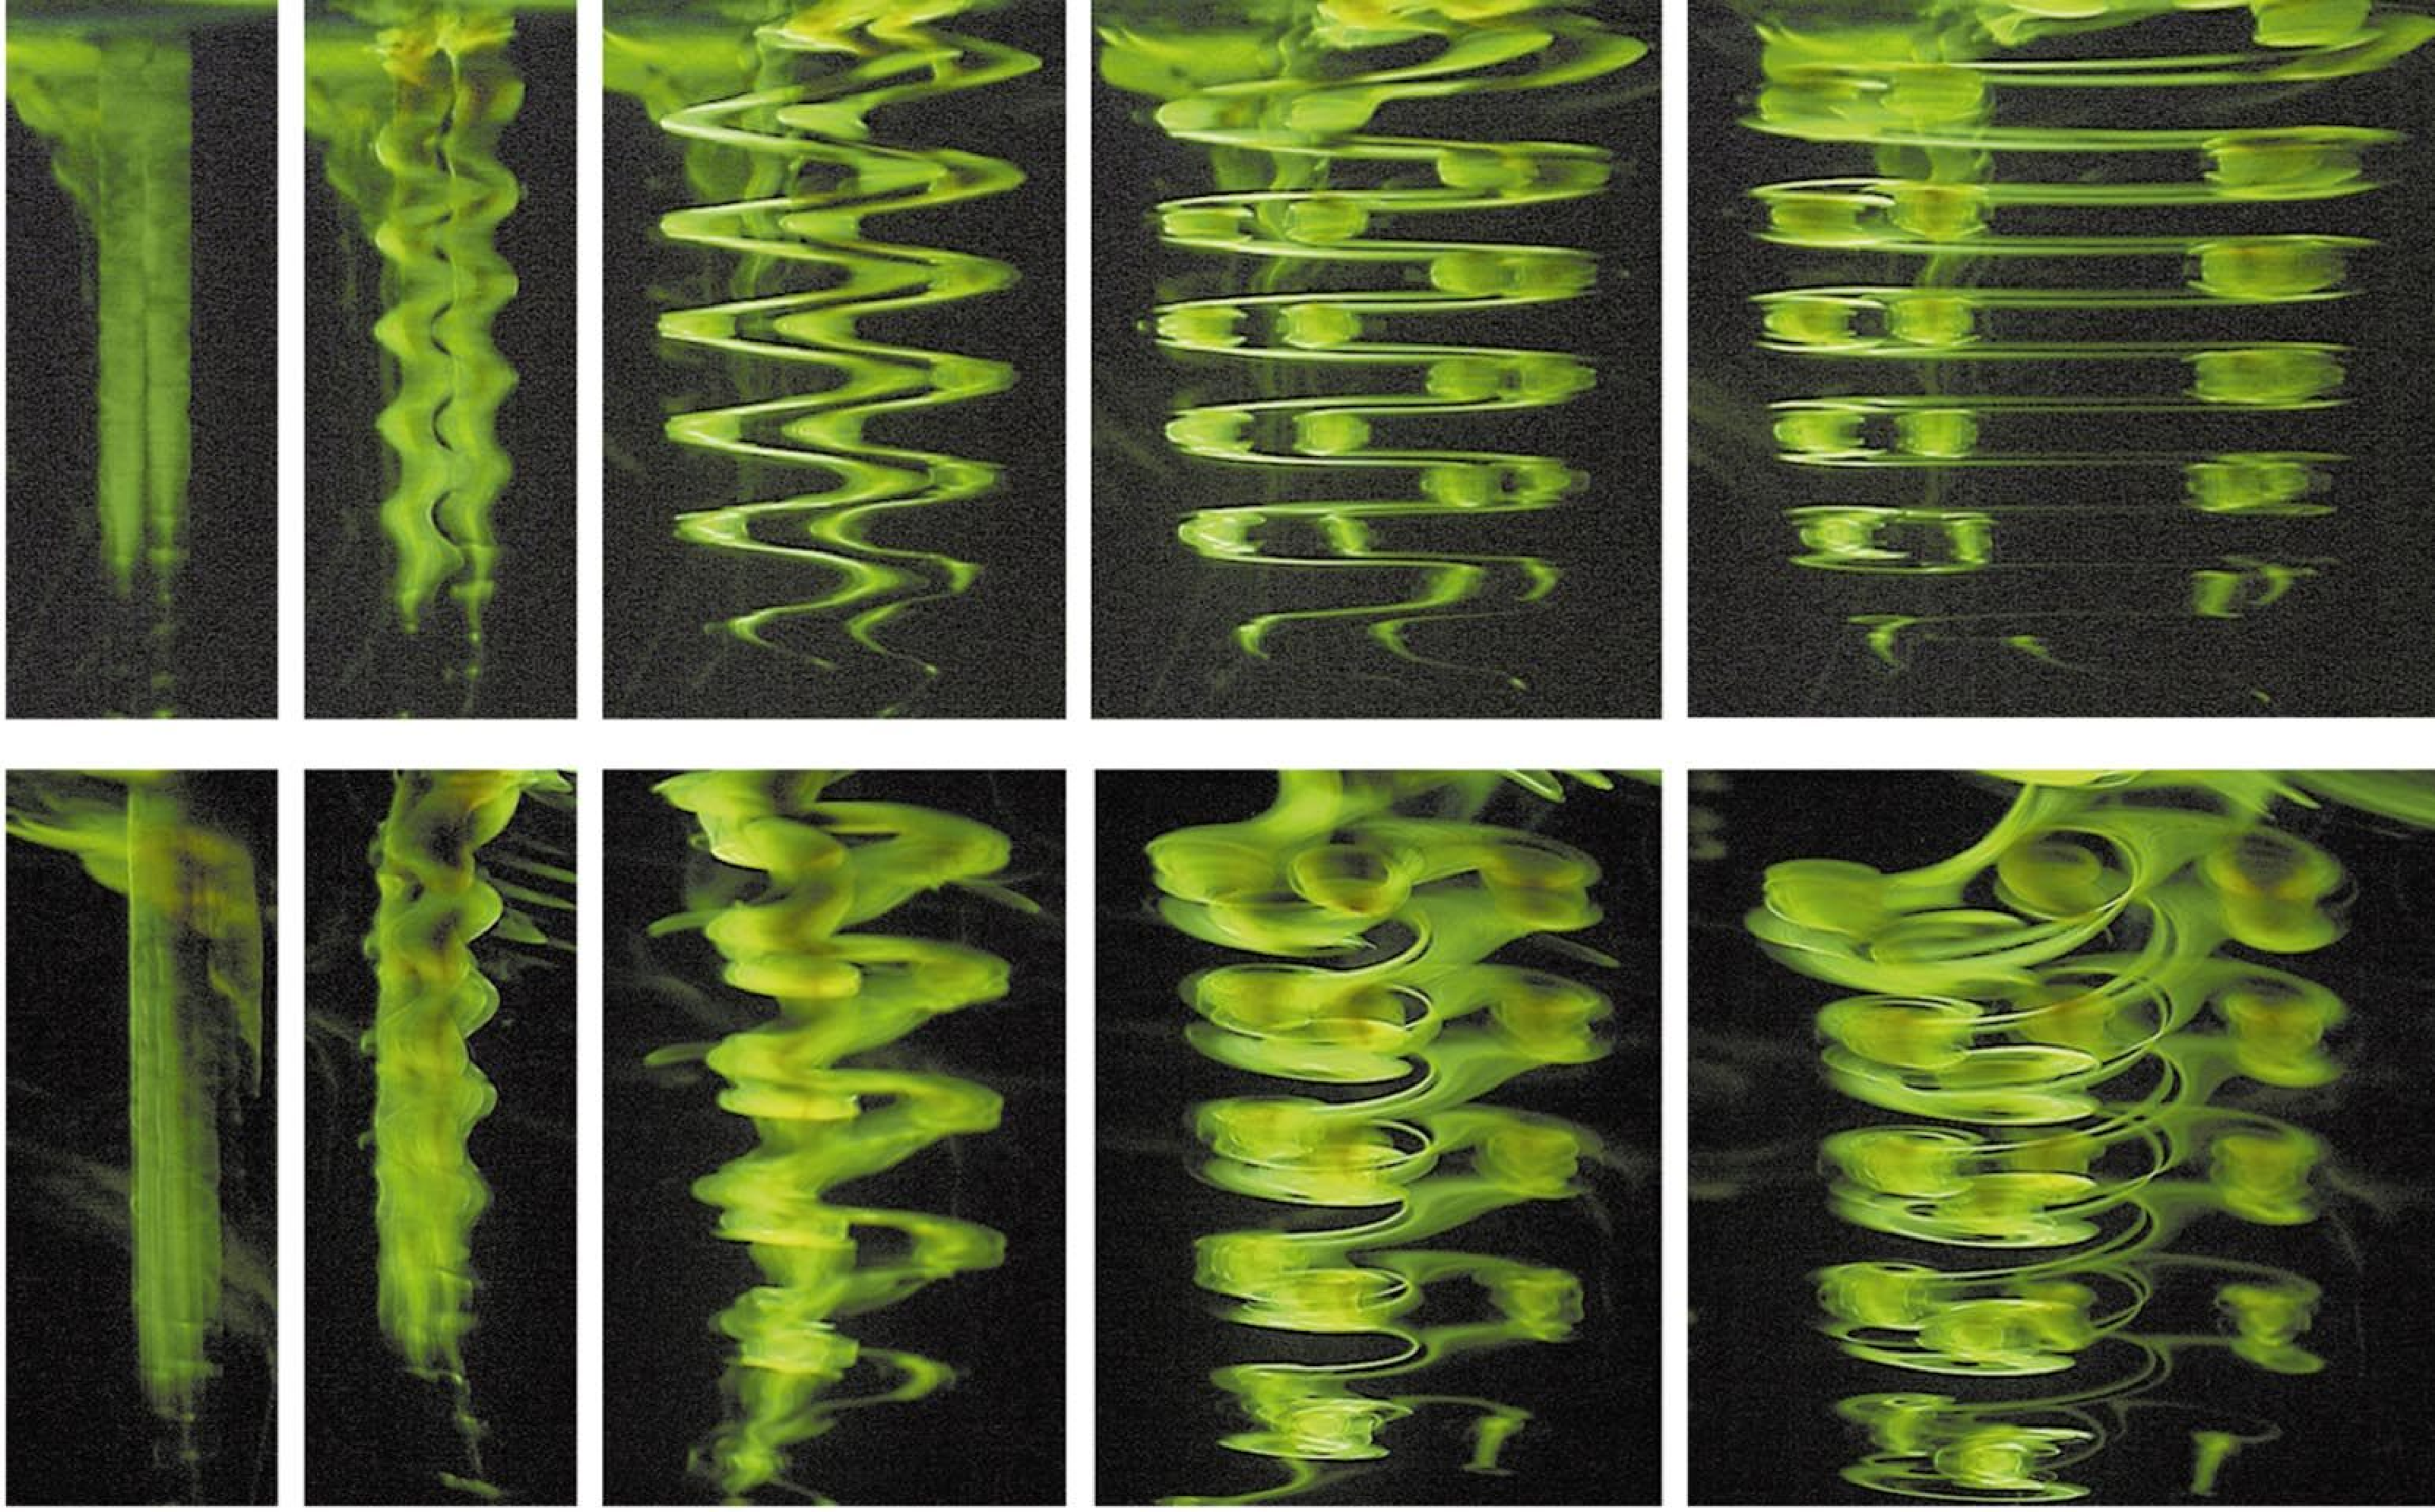
\includegraphics[width=\textwidth]{zigzag_experimental.pdf}
%\caption{(get permission from JFM for picture + caption) A sequence of frontal (top) and side (bottom) views showing the growth of the zigzag instability for $F_{h}=0.19$ and $Re=365$. From left to right the pictures are taken at $7,36,75,109,121,176$ seconds after the flaps have closed. The vortex pair is propogating to the left. In this experiment, tape has been applied to force the the natural wavelength of the instability to produce a clearer result.}
%\label{zigzag_experimental}
%\end{center}
%\end{figure}
Figure 10 of \cite{bc2000a} demonstrates the evolution for the zigzag instability for $F_{h}=0.19$ and $Re=365$. The structure of the vortices displays a zigzag like structure. Additionally, the anisotropy between the vertical and horizontal directions is quite clear. The periodic behaviour of the vortex pair is also evident. 

%BC also confirmed the results of the Japanese guys because they found that below $F_{h}=0.22$ the elliptical instability was suppressed by stratification. 

%Billant and Chomaz had experimentally observed this new instability which occured when $F_{h}<0.22$ 

Following up the experimental work, Billant and Chomaz provided a theoretical account of the zigzag instability starting from the Boussinesq equations \cite{bc2000b}. We will only discuss the main result of the paper as the paper is a very technical and long perturbation analysis. In the paper, they investigated the limit where $F_{h,v} = U/L_{h,v}N \ll 1$ and found that the zigzag motion was accounted for by combination of translation and rotation, which agrees with the experimental observations of \cite{bc2000a}. Additionally, they found that the most unstable vertical length scale of the zigzag instability should behave as $F_{v} \sim \mathcal{O}(1)$, i.e. $L_{v} \sim U/N$. This length is known as the buoyancy length scale (e.g. Waite \cite{waite2011}) and has proven to be a very important length scale in stratified fluid flow, as we shall discuss below. This emergence of the buoyancy length scale in their calculations, however,  should be treated with some care since Billant and Chomaz assumed that $F_{v}\ll 1$ and showed that $F_{v}\sim \mathcal{O}(1)$. 

In the third paper, Billant and Chomaz conducted a numerical linear stability analysis of the zigzag instability \cite{bc2000c}. In this study, they numerically solved the linear Boussinesq equations for the growth rate of the leading eigenmode for specific wavenumbers. We will not discuss the results details of the paper here as their paper forms the basis for much of this thesis and we will re-derive and discuss their results throughout the next three chapters. In the remainder of this chapter we derive the numerical equations that Billant and Chomaz used in \cite{bc2000c} and provide some more background information. In Chapter 3 we introduce and discuss the numerical technique of spectral methods used to solve the numerical equations. In Chapter 4 we extend the analysis of Billant and Chomaz to length scales well below the sub-buoyancy scale of $L_{b}\sim U/N$. 

\section{Formulation of the linear problem}
Following Billant and Chomaz \cite{bc2000c}, we consider the non-dimensional Boussinesq approximation to the Navier-Stokes equations in Cartesian co-ordinates 
\begin{align}
\frac{D\bm{u}}{Dt} = -\nabla p - \rho'\hat{\bm{e}}_{z} + \frac{1}{Re}\nabla^{2} \bm{u},\\
\nabla \cdot \bm{u}=0,\\
\frac{D\rho'}{Dt} -\frac{w}{F_{h}^{2}} = \frac{1}{ReSc}\nabla^{2} \rho',
\end{align}
where we have non-dimensionalised by the characteristic velocity $U$, length $R$, time-scale $R/U$, pressure $\rho_{0}U^{2}$, density $\rho_{0}U^{2}/gR$, and defined $Sc=\nu /\kappa$ as the Schmidt number, where $\kappa$ is the molecular diffusivity, $\rho_{0}$ is the background density, and $g$ is the gravitational constant. The Reynolds and horizontal Froude number are as defined above. The buoyancy frequency $N$, and hence the Froude number $F_{h}$, is assumed to be constant. 

In order to investigate the linear growth rate, we proceed as in Section 1.2 and expand the full velocity field as the sum of a basic state and a perturbation state:
\begin{align}
\bm{u} = \bm{u}_{0} + \tilde{\bm{u}},\\
p = p_{0} + \tilde{p},\\
\rho' = \rho'_{0} + \tilde{\rho}'.
\end{align}
The basic is chosen to be the Lamb-Chaplygin dipole which we will now discuss and explain how it provides a convenient theoretical model for the experiment by Billant and Chomaz \cite{bc2000a}.


\subsection{The Lamb-Chaplygin Dipole} 
As the basic state for linear stability analysis we use the Lamb-Chaplygin dipole in a comoving frame \cite{meleshko1994}. This dipole is a solution to the 2D inviscid Euler equations. This basic state is motivated by numerous laboratory experiments\cite{bc2000a,leweke1998}, as discussed above, which demonstrated that a vertically oriented Lamb-Chaplygin dipole is a good approximation to the vortex generated by two flaps closing in a tank of salt-stratified water. The dipole, in cylindrical coordinates, is given by the stream function
\begin{align}
\psi_{0}(r,\theta) = 
\begin{dcases}
-\frac{2}{\mu_{1}J_{0}(\mu_{1})}J_{1}(\mu_{1}r)\sin\theta & r\le 1,\\\label{lc_dipole_sf}
-r\left(1-\frac{1}{r^{2}}\right)\sin\theta & r>1 ,
\end{dcases}
\end{align}
and the corresponding vertical vorticity $\omega_{z0}=\nabla_{h}^{2}\psi_{0}$
\begin{align}
\omega_{z0}(r,\theta) = \
\begin{dcases}
\mu_{1}^{2}\psi_{0}(r,\theta) & r\le 1,\\
0 & r>1,
\end{dcases}
\end{align}
where $J_{0},J_{1}$ are the zero and first order Bessel functions, $\mu_{1}\approx 3.8317$ is the first root of $J_{1}$, and $\nabla_{h}$ is the horizontal Laplacian. The basic state velocity is purely horizontal and is given by $\bm{u}_{h0}=\nabla_{h}\psi_{0}\times\hat{\bm{e}}_{z}$. Recall that in the previous section, Billant and Chomaz found experimentally that $\omega = k^{2}\psi$ where $k=1.15$. Here we have that $\omega_{z0}=\mu_{1}^{2}\psi_{0}$. If we consider the dimensional version, we would have that $k^{2} = \mu_{1}^{2}/R^{2}$ where $R=3.6$ cm. This gives $k^{2} = 1.13 \text{ cm}^{-2}$ which corresponds very well with the experimental value of $1.15$. Fig.~\ref{lamb_dipole_plot} is a plot of the vorticity. 

\begin{figure}
\begin{center}
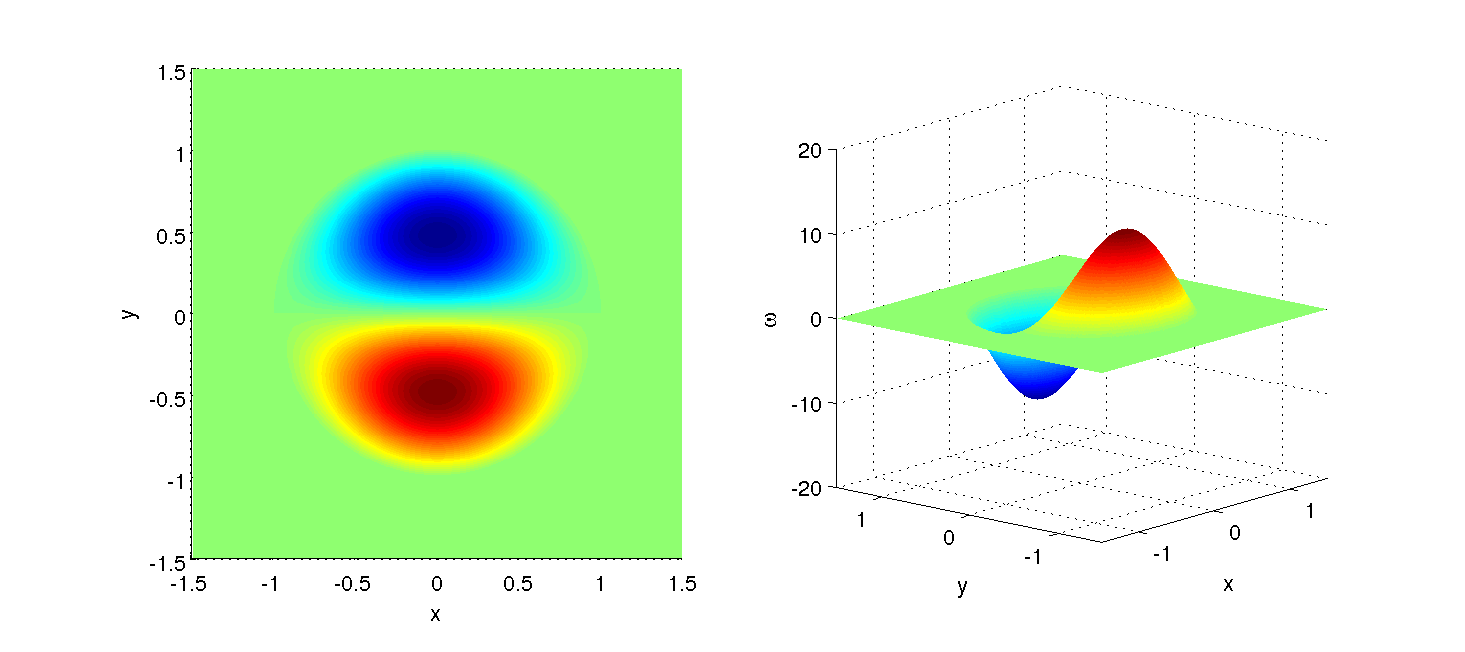
\includegraphics[width=\textwidth]{lamb_dipole}
\caption{The Lamb-Chaplygin dipole.}
\label{lamb_dipole_plot}
\end{center}
\end{figure}
Let us now discuss the derivation of this result, which was first written down by Lamb and investigated further, independently, by Chaplygin \cite{meleshko1994}. Although Lamb was the first to write down the above solution to the Euler equations, he did not provide any motivation for the derivation beyond it being an exact solution of the 2D steady Euler equations. However, a decade later, Lamb provided a slightly more in depth derivation motivating somewhat the study of this dipole. Independently, in Russia, Chaplygin provided a complete derivation and motivation for studying this dipole, although it remained unknown outside of Russia. Following \cite{meleshko1994} we repeat the key points of Chaplygin's argument. 

Recall that the steady 2D Euler equations can be written in terms of the stream function $\psi$ and a vorticity $\omega$ as
\begin{align}
\nabla^{2} \psi = - \omega.\label{vort_eq_chap}
\end{align}
To choose $\omega$, Chaplygin was motivated by the situation where we have a continuous vortex whose outer region is steady irrotational flow while the inner region is a translating vortex. Recall that the potential function for a flow outside a cylinder is
\begin{align}
\psi = v_{0}\left(r - \frac{a^{2}}{r}\right)\sin\theta ,
\end{align}
where $a$ is the radius of the dipole and $v_{0}$ is the propagation velocity. 

Inside the radius $a$, Chaplygin chose the vorticity to be $\omega = n^{2}\psi$ where $n$ is a constant. In polar coordinates (\ref{vort_eq_chap}) becomes
\begin{align}
\frac{\partial^{2}\psi}{\partial r^{2}} + \frac{1}{r}\frac{\partial \psi}{\partial r} + \frac{1}{r^{2}}\frac{\partial^{2}\psi}{\partial \theta^{2}} =  n^{2}\psi,
\end{align}
which we can guess at a solution of the form $\psi(r,\theta) = Z(r)\sin\theta$. Although Chaplygin did not provide specific motivation for choosing this specific vorticity, the above equation has a form that is similar to the irrotational flow outside the dipole and this makes the matching conditions simple. The resulting equation for $Z(r)$ is the well known Bessel equation \cite{meleshko1994} and after working through the algebra, one obtains (\ref{lc_dipole_sf}). Chaplygin also investigated the resulting pressure field produced by the dipole and was able to compute the circulation of the dipole \cite{meleshko1994}. Unlike Lamb, he also considered a generalisation of the above where the dipole is no longer symmetric about the x-axis. The corresponding vorticity in this case is given by
\begin{align}
\omega = n^{2}(\psi - \lambda),
\end{align}
where $\lambda$ is an arbitrary parameter where $\lambda=0$ is a completely symmetric dipole and $\lambda\rightarrow\infty$ corresponds to a completely asymmetric dipole. Here, again, Chaplygin investigated fully the pressure and circulation produced by this dipole. Additionally, in the same set of papers, Chaplygin also investigated the case of the dipole in rotating fluid, which was independently rediscovered 80 years later. Full details of this derivation are in \cite{meleshko1994}.


\section{Scaling analysis}
We have mentioned two dimensionless numbers in stratified flow, the Reynolds number and the Froude number. Both these dimensionless numbers arise when comparing the relative sizes of various terms in the Navier-Stokes equations. Depending on what aspect of a problem we are looking at, these numbers can appear in different places when we choose different scalings. We will now discuss some of the scaling arguments that have been used in stratified flow as it can provide insights into what mechanisms underlie the transition to and evolution of turbulence. A comprehensive review of scaling in stratified turbulence is provided in a recent review by Riley and Lindborg \cite{rileylindborg2013} and we will discuss the important scaling arguments therein. 

For reference, we reproduce the Boussinesq equations here 
\begin{align}
\frac{\partial \textbf{u}_{h}'}{\partial t'} + \textbf{u}_{h}'\cdot\nabla'_{h}\textbf{u}_{h}'+u_{z}'\frac{\partial \textbf{u}_{h}'}{\partial z'} &= -\frac{1}{\rho_{0}}\nabla'_{h}p' + \nu \nabla'^{2}\textbf{u}_{h},\\
\frac{\partial u_{z}'}{\partial t'} + \textbf{u}_{h}'\cdot\nabla'_{h}u_{z}'+u_{z}'\frac{\partial u_{z}'}{\partial z'} &= -\frac{1}{\rho_{0}}\frac{\partial p'}{\partial z'} - \frac{\rho' g}{\rho_{0}} + \nu \nabla'^{2}u_{z},\\
\nabla'_{h}\cdot\textbf{u}_{h}' + \frac{\partial u_{z}'}{\partial z'} &=0,\\
\frac{\partial \rho'}{\partial t'} + \textbf{u}_{h}'\cdot\nabla_{h}'\rho' + u_{z}'\frac{\partial \rho'}{\partial z'} + \frac{\partial \rho}{\partial z'}u_{z}'&=\kappa\nabla^{2}\rho ',
\end{align}
where the primed quantities denote the dimensional quantities. 

As a starting point, we produce a scaling argument that separates the horizontal and vertical directions. As we saw in the experiment of Billant and Chomaz \cite{bc2000a}, in the zigzag instability there was a clear separation between the vertical and horizontal scales. This difference in the vertical and horizontal directions suggests defining two length scales, the horizontal length scale $L_{h}$ and the vertical length scale $L_{v}$. Associated with this separation we introduce the horizontal velocity scale $U$ and the vertical velocity scale $W$. The resulting scaling is
\begin{align}
x'=L_{h}x,\qquad y' =L_{h}y, \qquad z'=L_{v}z, \qquad \textbf{u}_{h}' = U\textbf{u}, \qquad u_{z}' = Wu_{z}.
\end{align}
We also define another useful quantity that plays an important role in the scaling of stratified flows, the aspect ratio
\begin{align}
\delta = \frac{L_{v}}{L_{h}},
\end{align}
which measures how anisotropic the length scales are. For the time scale, we choose the advective time scale 
\begin{align}
t' = \frac{L_{h}}{U}t,
\end{align}
which is the characteristic time of a vortex to be advected around the characteristic length \cite{rileylelong2000,bc2001,lilly1983}. Following these references the pressure scales such that the horizontal pressure gradient is the same order as the advection terms and density scales from approximate hydrostatic balance
\begin{align}
p' = \rho_{0}U^{2}p, \qquad \rho' = \frac{U^{2}\rho_{0}}{gL_{v}}\rho.
\end{align}
The only quantity left unspecified is the vertical velocity which can be determined by setting balancing the linear terms and the time derivative terms in the density equation \cite{bc2001,rileylelong2000} giving the scaling 
 \begin{align}
u_{z}' = U\frac{F_{h}^{2}}{\delta}u_{z}.
\end{align}
This scaling now leads to the following set of equations \cite{rileylindborg2013}
\begin{align}
\frac{\partial \textbf{u}_{h}}{\partial t} + \textbf{u}_{h}\cdot\nabla_{h}\textbf{u}_{h}+\frac{F_{h}^{2}}{\alpha^{2}}u_{z}\frac{\partial \textbf{u}_{h}}{\partial z} &= -\nabla_{h}p + \frac{1}{\Re}\left(\nabla^{2}_{h}\textbf{u}_{h}+\frac{1}{\alpha^{2}}\frac{\partial^{2}\textbf{u}_{h}}{\partial z^{2}}\right),\\
F_{h}^{2}\left(\frac{\partial u_{z}}{\partial t} + \textbf{u}_{h}\cdot\nabla_{h}u_{z}+\frac{F_{h}^{2}}{\alpha^{2}}u_{z}\frac{\partial u_{z}}{\partial z}\right) &= -\frac{\partial p}{\partial z} - \rho + \frac{F_{h}^{2}}{\Re}\left(\frac{1}{\alpha^{2}}\frac{\partial u_{z}}{\partial z^{2}} + \nabla^{2}_{h}u_{z}\right),\\
\nabla_{h}\cdot\textbf{u}_{h} + \frac{F_{h}^{2}}{\alpha^{2}}\frac{\partial u_{z}}{\partial z} &=0,\\
\frac{\partial \rho}{\partial t} + \textbf{u}_{h}\cdot\nabla_{h}\rho + \frac{F_{h}^{2}}{\alpha^{2}}u_{z}\frac{\partial \rho}{\partial z} &= u_{z} + \frac{1}{\Re Sc}\left(\frac{1}{\alpha^{2}}\frac{\partial^{2}\rho}{\partial z^{2}} + \nabla^{2}_{h}\rho\right),
\end{align} 
where 
\begin{align}
\Re = \frac{UL_{h}}{\nu}, \qquad F_{h} = \frac{U}{L_{h}N},\qquad Sc = \frac{\nu}{\kappa}.
\end{align}
Lilly was the first to write these equations down although he assumed isotropy, i.e. $\delta=1$. 

Let us now investigate the limit of strong stratification, i.e. $F_{h}\rightarrow 0$ but let us leave the behaviour of $F_{h}/\delta$ undetermined. Additionally, let us consider $\Re\gg 1$ and following \cite{rileylindborg2013} ignore the diffusion terms that only depend on $Re$ but not $Re\delta^{2}$.  This results in the following equations 
\begin{align}
\frac{\partial \textbf{u}_{h}}{\partial t} + \textbf{u}_{h}\cdot\nabla_{h}\textbf{u}_{h}+\frac{F_{h}^{2}}{\alpha^{2}}u_{z}\frac{\partial \textbf{u}_{h}}{\partial z} &= -\nabla_{h}p + \frac{1}{\Re}\frac{1}{\alpha^{2}}\frac{\partial^{2}\textbf{u}_{h}}{\partial z^{2}},\\
0&= -\frac{\partial p}{\partial z} - \rho, \\
\nabla_{h}\cdot\textbf{u}_{h}+ \frac{F_{h}^{2}}{\alpha^{2}}\frac{\partial u_{z}}{\partial z} &=0,\\
\frac{\partial \rho}{\partial t} + \textbf{u}_{h}\cdot\nabla_{h}\rho + \frac{F_{h}^{2}}{\alpha^{2}}u_{z}\frac{\partial \rho}{\partial z} &= u_{z} + \frac{1}{\Re Sc}\frac{1}{\alpha^{2}}\frac{\partial^{2}\rho}{\partial z^{2}} .
\end{align} 
It was initially assumed by Lilly \cite{lilly1983} and Riley et al.\cite{rileylelong2000} that as $F_{h}\rightarrow 0$ then so does $F_{h}/\delta$. Thus the resulting equations are 
\begin{align}
\frac{\partial \textbf{u}_{h}}{\partial t} + \textbf{u}_{h}\cdot\nabla_{h}\textbf{u}_{h} &= -\nabla_{h}p + \frac{1}{\Re}\frac{1}{\alpha^{2}}\frac{\partial^{2}\textbf{u}_{h}}{\partial z^{2}},\\
0&= -\frac{\partial p}{\partial z} - \rho  \\
\nabla_{h}\cdot\textbf{u}_{h} &=0\\
\frac{\partial \rho}{\partial t} + \textbf{u}_{h}\cdot\nabla_{h}\rho &= \frac{1}{\Re Sc}\frac{1}{\alpha^{2}}\frac{\partial^{2}\rho}{\partial z^{2}} 
\end{align} 
Notice that in these resulting equations, the horizontal and vertical velocities have become almost completely decoupled. They are not completely decoupled because there is still dependence through the pressure term. However this decoupling led Lilly to conjecture that stratified turbulence in the strong stratification limit will resemble layerwise 2D turbulence with an inverse energy cascade\cite{lilly1983}. However, subsequent numerical simulations of stratified turbulence were not able to reproduce an inverse cascade, raising doubts about the applicability of Lilly's equations (e.g. Herring and Metais \cite{metais1989}, Waite and Bartello \cite{waitebartello2004}).


Building on the work of Lilly \cite{lilly1983} and Riley et al.\cite{rileylelong2000}, Billant and Chomaz \cite{bc2001} modified the argument suggesting that instead $F_{h}/\delta\rightarrow 1$, not $0$, as $F_{h}\rightarrow 1$. This scaling analysis leads to $L_{v} \sim U/N$ which is the dominant vertical scale for the zigzag instability. The resulting equations are

\begin{align}
\frac{\partial \textbf{u}_{h}}{\partial t} + \textbf{u}_{h}\cdot\nabla_{h}\textbf{u}_{h}+u_{z}\frac{\partial \textbf{u}_{h}}{\partial z} &= -\nabla_{h}p + \frac{1}{\Re}\frac{1}{\alpha^{2}}\frac{\partial^{2}\textbf{u}_{h}}{\partial z^{2}},\\
0&= -\frac{\partial p}{\partial z} - \rho, \\
\nabla_{h}\cdot\textbf{u}_{h}+ \frac{\partial u_{z}}{\partial z} &=0,\\
\frac{\partial \rho}{\partial t} + \textbf{u}_{h}\cdot\nabla_{h}\rho + u_{z}\frac{\partial \rho}{\partial z} &= u_{z} + \frac{1}{\Re Sc}\frac{1}{\alpha^{2}}\frac{\partial^{2}\rho}{\partial z^{2}}. 
\end{align} 
The assumption that $F_{h}/\delta \rightarrow 1$ can be rewritten to state that $L_{v} \sim U/N$, which is the buoyancy scale. In this case, there is no decoupling between the horizontal and vertical directions and the advection terms and incompressibility condition are fully three-dimensional. 

%\subsection{Stratified Turbulence}
%In this thesis we focus on the linear stability and the transition to stratified turbulence, but not on stratified turbulence itself however it worth making a few brief remarks. For an in-depth recent review, see Lindborg and Riley \cite{rileylindborg2013} which contains a thorough review of recent process made in stratified turbulence in experimental, theoretical, and numerical results.
%
%Experimental results by Nastrom and Gage \cite{nastrom1985} analysing data from airplanes have shown that stratified turbulence in the atmosphere exhibits the scaling of the horizontal energy spectrum as $k_{h}^{-3}$ at large horizontal scales and as $k_{h}^{-5/3}$ as small horizontal scales. The $k_{h}^{-3}$ spectrum is well known in the quasi-geostrophic community (source?). The $k_{h}^{-5/3}$ is the well known \cite{lesieur} scaling of isotropic homogeneous turbulence derived by Kolmogorov in the 1940s. The appearance of this scaling is surprising since anisotropy, as we have discussed, is very important in stratified flows. One possible theory, proposed by Lindborg \cite{lindborg2006}, is that the buoyancy length $U/N$, here meaning the length scale of the eddies within the flow, plays the important role in governing the evolution of the turbulence. However many open questions remain (cite?).
%

